% Options for packages loaded elsewhere
\PassOptionsToPackage{unicode}{hyperref}
\PassOptionsToPackage{hyphens}{url}
%
\documentclass[
  ignorenonframetext,
]{beamer}
\title{Predicting the Risk of Recurrent MI}
\subtitle{SIBS Hackathon Presentation}
\author{Kevin Krupa, Lucy Liu, Kendall McClellan, Connor McNeill}
\date{July 21, 2022}
\institute{NCSU-Duke Summer Institute in Biostatistics}

\usepackage{pgfpages}
\setbeamertemplate{caption}[numbered]
\setbeamertemplate{caption label separator}{: }
\setbeamercolor{caption name}{fg=normal text.fg}
\beamertemplatenavigationsymbolsempty
% Prevent slide breaks in the middle of a paragraph
\widowpenalties 1 10000
\raggedbottom
\setbeamertemplate{part page}{
  \centering
  \begin{beamercolorbox}[sep=16pt,center]{part title}
    \usebeamerfont{part title}\insertpart\par
  \end{beamercolorbox}
}
\setbeamertemplate{section page}{
  \centering
  \begin{beamercolorbox}[sep=12pt,center]{part title}
    \usebeamerfont{section title}\insertsection\par
  \end{beamercolorbox}
}
\setbeamertemplate{subsection page}{
  \centering
  \begin{beamercolorbox}[sep=8pt,center]{part title}
    \usebeamerfont{subsection title}\insertsubsection\par
  \end{beamercolorbox}
}
\AtBeginPart{
  \frame{\partpage}
}
\AtBeginSection{
  \ifbibliography
  \else
    \frame{\sectionpage}
  \fi
}
\AtBeginSubsection{
  \frame{\subsectionpage}
}
\usepackage{amsmath,amssymb}
\usepackage{lmodern}
\usepackage{iftex}
\ifPDFTeX
  \usepackage[T1]{fontenc}
  \usepackage[utf8]{inputenc}
  \usepackage{textcomp} % provide euro and other symbols
\else % if luatex or xetex
  \usepackage{unicode-math}
  \defaultfontfeatures{Scale=MatchLowercase}
  \defaultfontfeatures[\rmfamily]{Ligatures=TeX,Scale=1}
  \setmainfont[]{Arial}
\fi
\usetheme[]{Frankfurt}
\usefonttheme{serif} % use mainfont rather than sansfont for slide text
% Use upquote if available, for straight quotes in verbatim environments
\IfFileExists{upquote.sty}{\usepackage{upquote}}{}
\IfFileExists{microtype.sty}{% use microtype if available
  \usepackage[]{microtype}
  \UseMicrotypeSet[protrusion]{basicmath} % disable protrusion for tt fonts
}{}
\makeatletter
\@ifundefined{KOMAClassName}{% if non-KOMA class
  \IfFileExists{parskip.sty}{%
    \usepackage{parskip}
  }{% else
    \setlength{\parindent}{0pt}
    \setlength{\parskip}{6pt plus 2pt minus 1pt}}
}{% if KOMA class
  \KOMAoptions{parskip=half}}
\makeatother
\usepackage{xcolor}
\IfFileExists{xurl.sty}{\usepackage{xurl}}{} % add URL line breaks if available
\IfFileExists{bookmark.sty}{\usepackage{bookmark}}{\usepackage{hyperref}}
\hypersetup{
  pdftitle={Predicting the Risk of Recurrent MI},
  pdfauthor={Kevin Krupa, Lucy Liu, Kendall McClellan, Connor McNeill},
  hidelinks,
  pdfcreator={LaTeX via pandoc}}
\urlstyle{same} % disable monospaced font for URLs
\newif\ifbibliography
\usepackage{graphicx}
\makeatletter
\def\maxwidth{\ifdim\Gin@nat@width>\linewidth\linewidth\else\Gin@nat@width\fi}
\def\maxheight{\ifdim\Gin@nat@height>\textheight\textheight\else\Gin@nat@height\fi}
\makeatother
% Scale images if necessary, so that they will not overflow the page
% margins by default, and it is still possible to overwrite the defaults
% using explicit options in \includegraphics[width, height, ...]{}
\setkeys{Gin}{width=\maxwidth,height=\maxheight,keepaspectratio}
% Set default figure placement to htbp
\makeatletter
\def\fps@figure{htbp}
\makeatother
\setlength{\emergencystretch}{3em} % prevent overfull lines
\providecommand{\tightlist}{%
  \setlength{\itemsep}{0pt}\setlength{\parskip}{0pt}}
\setcounter{secnumdepth}{-\maxdimen} % remove section numbering
\AtBeginSection[]
{
 \begin{frame}<beamer>
 \frametitle{Outline}
 \tableofcontents[currentsection]
 \end{frame}
}

\definecolor{darkred}{rgb}{0.8,0,0}
%\setbeamercolor{section number projected}{bg=darkred, fg=darkred}
%\setbeamercolor{structure}{bg=darkred}

\usepackage{amsmath}
\usepackage{amssymb}
\usepackage{amsthm}

\usepackage{lmodern}
\renewcommand*\familydefault{\sfdefault} %% Only if the base font of the document is to be sans serif
\usepackage[T1]{fontenc}
\usepackage[lm]{sfmath}

\renewcommand{\qedsymbol}{\rule{0.7em}{0.7em}}
\ifLuaTeX
  \usepackage{selnolig}  % disable illegal ligatures
\fi

\begin{document}
\frame{\titlepage}

\hypertarget{introduction}{%
\section{Introduction}\label{introduction}}

\begin{frame}{Background}
\protect\hypertarget{background}{}
\begin{itemize}
\item
  Bullet 1
\item
  Bullet 2
\item
  Bullet 3
\end{itemize}
\end{frame}

\begin{frame}{Research Question}
\protect\hypertarget{research-question}{}
\begin{block}{Question 1}
What can we look at either during admission or the hospital stay in patients post-heart attack (myocardial infarction) to predict the risk of having a relapse?
\end{block}

\begin{block}{Question 2}
Which risk prediction model is best at predicting a recurrent heart attack?
\end{block}
\end{frame}

\begin{frame}[fragile]{Missing Data}
\protect\hypertarget{missing-data}{}
\begin{itemize}
\item
  7.6\% missing values
\item
  Used \texttt{mice} library in \texttt{R}

  \begin{itemize}
  \item
    Predictive Mean Modeling
  \item
    1700 completed observations instead of 0!
  \end{itemize}
\end{itemize}
\end{frame}

\hypertarget{descriptive-analysis}{%
\section{Descriptive Analysis}\label{descriptive-analysis}}

\begin{frame}{Response Variable Correlation}
\protect\hypertarget{response-variable-correlation}{}
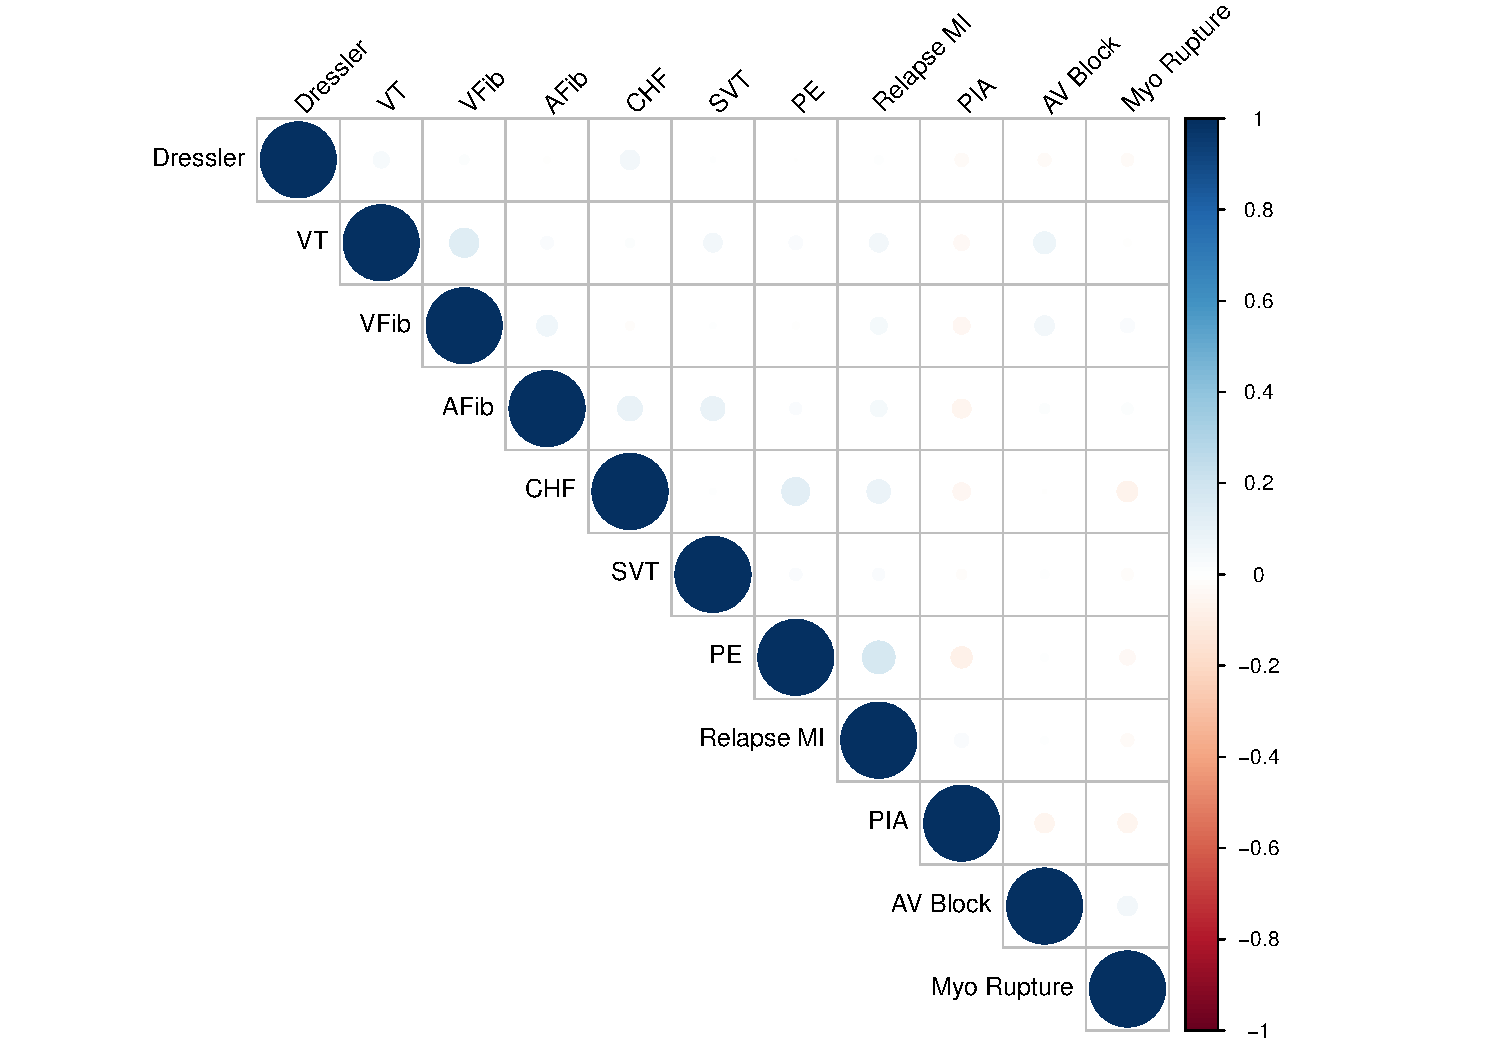
\includegraphics{sibs-hackathon-presentation_files/figure-beamer/ResVarCorrPlot-1.pdf}
\end{frame}

\hypertarget{inferential-analysis}{%
\section{Inferential Analysis}\label{inferential-analysis}}

\begin{frame}{Model Building}
\protect\hypertarget{model-building}{}
Logistic regression is the basis

\begin{itemize}
\item
  Response variable (recurrent MI) is binary
\item
  Multiple predictors

  \begin{itemize}
  \item
    \(>100\) covariates to begin
  \item
    Several removed from consideration due to missingness
  \item
  \end{itemize}
\end{itemize}
\end{frame}

\begin{frame}[fragile]{Model Building}
\protect\hypertarget{model-building-1}{}
Two methods to select significant predictors:

\begin{enumerate}
\item
  Backwards Elimination using AIC (\texttt{stepAIC})
\item
  Elastic Net Penalized Regression (\texttt{glmnet})
\end{enumerate}

Methods will pick predictors and build model
\end{frame}

\begin{frame}{Model}
\protect\hypertarget{model}{}
\[ REC\_IM = \beta_0 + \beta_1 x_1 \]

\textbackslash end\{subsection\}
\end{frame}

\hypertarget{discussion}{%
\section{Discussion}\label{discussion}}

\hypertarget{conclusion}{%
\section{Conclusion}\label{conclusion}}

\begin{frame}{}
\protect\hypertarget{section}{}
\begin{block}{}
\begin{center}
\Large{Questions??}
\end{center}
\end{block}
\end{frame}

\end{document}
